\chapter{Muon Detection} \label{sec:detection}

Muons can be measured by the energy losses along their propagated track, each producing a particle cascade.
While the bare muon also produces a signal, the main signature is produced by the secondaries of the energy losses.
Here the main detection techniques of muons for cosmic-ray detectors and neutrino telescopes are presented.

\section{Detection principles}

The \textbf{Cherenkov Effect} \cite{Cherenkov34} describes the optical light produced by a charged particles propagating faster than the speed of light through a medium.
Due to the through-going charged particle, the medium gets polarized and creates a signal.
These signals are emitted coherently when the charged particle propagates faster than the speed of light in this medium, creating a Cherenkov cone with an opening angle of $\cos \theta = 1/\beta n$ similar to a hypersonic cone of an Airforce jet.
$n$ is the refraction index that also depends on the wavelength.
The Frank-Tamm formula \cite{FrankTamm37} describing the spectrum of the emitted Cherenkov photons has a $1/\lambda^2$ dependency, with the wavelength $\lambda$, and is therefore UV-divergent (neglecting the suppressing contribution of the refraction index).
Focusing on the optical wavelength and the medium ice, around \num{400} Cherenkov photons are emitted per centimeter with the main contribution of around \SI{400}{nm} (blue light).
The energy loss caused by the Cherenkov effect is around \SI{170}{eV/cm} which is four orders of magnitudes below the minimum Ionization loss of \SI{2}{MeV.\per.cm} and is therefore negligible for the energy loss during the propagation.
The Cherenkov light can be measured with Photomultiplier Tubes (PMTs) with the advantage of a wide collection area useful in water tanks but with the disadvantage of demanding high voltages.
Alternatively, the light can be measured with Silicon Photo Multiplier (SiPM) being able to operate without high voltages but only having a small collection area and therefore only applicable when the light is guided to them.

The \textbf{Askaryan Effect} \cite{Askaryan62} describes the radio signal caused by the relativistic propagation of a particle cascade.
In principle, the radio signal is produced by the geomagnetic and the Askaryan effect, but it is commonly known as the Askaryan effect.
The geomagnetic effect describes the separation of positrons and electrons during an electromagnetic cascade due to the geomagnetic field.
Due to the high number of shower particles, this creates a dipole perpendicular to the shower axis changing over time as the shower increases to its $X_{\text{max}}$ and then decreases.
Since there are only atomic electrons and no positrons, these electrons of a medium get knocked-out by the shower particles and the shower front gets charged negatively leaving the positively charged ions behind.
This charge imbalance along the shower axis is also changing over time as the shower develops which is considered as the Askaryan effect.
Both effects are just measurable because the particle cascade propagates faster than the speed of light in the medium thus producing a coherent radio signal at the Cherenkov angle.
For air showers, the radio signal is mainly produced by the geomagnetic effect while for more dense media, like ice, the Askaryan effect produces the dominant radio signal.
Only the highest energetic particle showers ($>\si{EeV}$) produce a sufficient amount of electrons and positrons and thereby a detectable radio signal.
The energy loss of \SI{18}{MeV} for an EeV shower due to this effect is even more negligible compared to the Cherenkov radiation.
The radio signal with wavelengths of a meter has a much higher attenuation length of about a kilometer in ice compared to \SI{100}{m} for optical light.

Even before the radio signal, Askaryan predicted an \textbf{acoustic signal} produced by high energetic cascades \cite{Askaryan57Acoustic}.
The huge amount of high energy charged particles inside the small shower region increases the energy and thereby the temperature of the medium in this area.
The heated region expands and creates an acoustic wave with a maximum frequency at \SI{10}{kHz}.
Through the coherent superposition of the sound waves, an acoustic signal perpendicular to the particle shower is produced that can be measured \cite{Lahmann16Acustic}.
Similar to the radio signal the attenuation length is on the order of a kilometer making both techniques interesting for rare events requiring huge detection volumes.

The \textbf{fluorescence effect} in general describes atoms or molecules that get excited and thus emitting optical light.
In the context of particle detectors, this is mainly used in scintillator detectors where the charged particle excites the scintillator material when passing through which emits light.
While the scintillation area can have a size of $\mathcal{O}(m^2)$, the emitted light can then be guided to a detector that just needs a small collection area, like an SiPM.
Besides this use of the fluorescence effect, the fluorescence light is used in the detection of the excited nitrogen molecules in the atmosphere caused by the huge number of high energetic particles in the shower \cite{Keilhauer12Fluorescence}.
The emitted fluorescence light at each shower depth is equivalent to the energy loss per distance making the energy of the shower extractable via the integral of the longitudinal shower profile.
Another type is the luminescence light which is used in searches of magnetic monopoles with neutrino telescopes, where the radio-luminescence induced by these highly ionizing particles has become a field of research \cite{Pollmann19Luminescence}.

%
% 
% small seperation between the chapters
%
%

\section{Air Shower Detectors}

The different signals an air shower produces are measured with multiple approaches, from the direct detection of the different shower particles at high altitudes over the muon detection at the surface to the fluorescence or radio signal besides the shower axis.

\subsection{$\gamma$-Ray induced Air Shower Detectors}

Extended air shower Arrays (EAS-Arrays) are placed at high altitudes, ideally near the typical maximum of the shower profile $X_{\mathrm{max}}$ to measure most of the produced particles inside the detector.
One approach is using a dense array of closed tanks filled with purified water.
Through-going charged particles of the shower produce Cherenkov light inside the water, which can be detected with optical sensors mainly PMTs.
Currently, the most sensitive observatory is the HAWC detector \cite{HAWC17} operating at an altitude of \SI{4.1}{km} above sea level (asl) in the Sierra Negra, Mexico.
Inside an area of \SI{22000}{\square\meter}, 300 cylindric tanks are placed each containing around \SI{200}{\cubic\meter} of water with 4 PMTs at the bottom measuring the Cherenkov light.
The upcoming LHAASO experiment in Tibet \cite{LHAASO19} will increase the sensitivity for air showers due to the higher altitude at \SI{4400}{m} asl.
Although EAS-Arrays are mainly designed to measure $\gamma$-ray induced air showers, one can also use them to analyze cosmic-ray induced showers in the PeV range around the \textit{knee} \cite{HAWC17CRSpectrum}.
Muons can be identified as they reach the ground of the detector producing light along their full track, while electrons will lose nearly all of their energy during their propagation through around \SI{4}{m} of water from the top of a tank to the bottom creating a uniform light pool.

Another type of telescope that was mainly developed for gamma astronomy but is also used to study cosmic-ray physics are imaging air Cherenkov telescopes (IACTs).
The detection techniques of both types of gamma telescope designs are illustrated in \figref{fig:detect_swgo}.
Hereby, the relativistic particles of an air shower are not measured directly, but indirectly via the Cherenkov light, they produce in the atmosphere, which can be also measured at moderate altitudes.
The current most sensitive telescopes are the HESS \cite{HESS20}, MAGIC \cite{MAGIC16II} and VERITAS \cite{VERITAS15Science} telescopes operating at \SI{1800}{m} \SI{2200}{m}, \SI{1300}{m} asl. respectively.
Electromagnetic or hadronic showers produce elliptical camera pictures with an additional spread-out for hadronic showers due to the higher transverse momentum of the hadronic interaction products.
Compared to that, muons produce a ring-like signature when propagating to the ground near the telescope.
Using this unique signature, IACT arrays measuring the same hadronic shower in multiple telescopes as well as the muons can give further insights into the muon flux produced in air showers \cite{Mitchell19MuonIACT}.
However, this approach will only work with an array of many telescopes as will be built in the upcoming CTA observatory \cite{CTA19Science}.
Compared to the closed tanks of EAS-Arrays with a duty cycle of nearly \SI{100}{\%}, IACTs can only operate at clear, moonless nights limiting their duty cycle to \SI{20}{\%}.
\begin{figure}
    \centering
    \begin{subfigure}{0.9\textwidth}
        \centering
        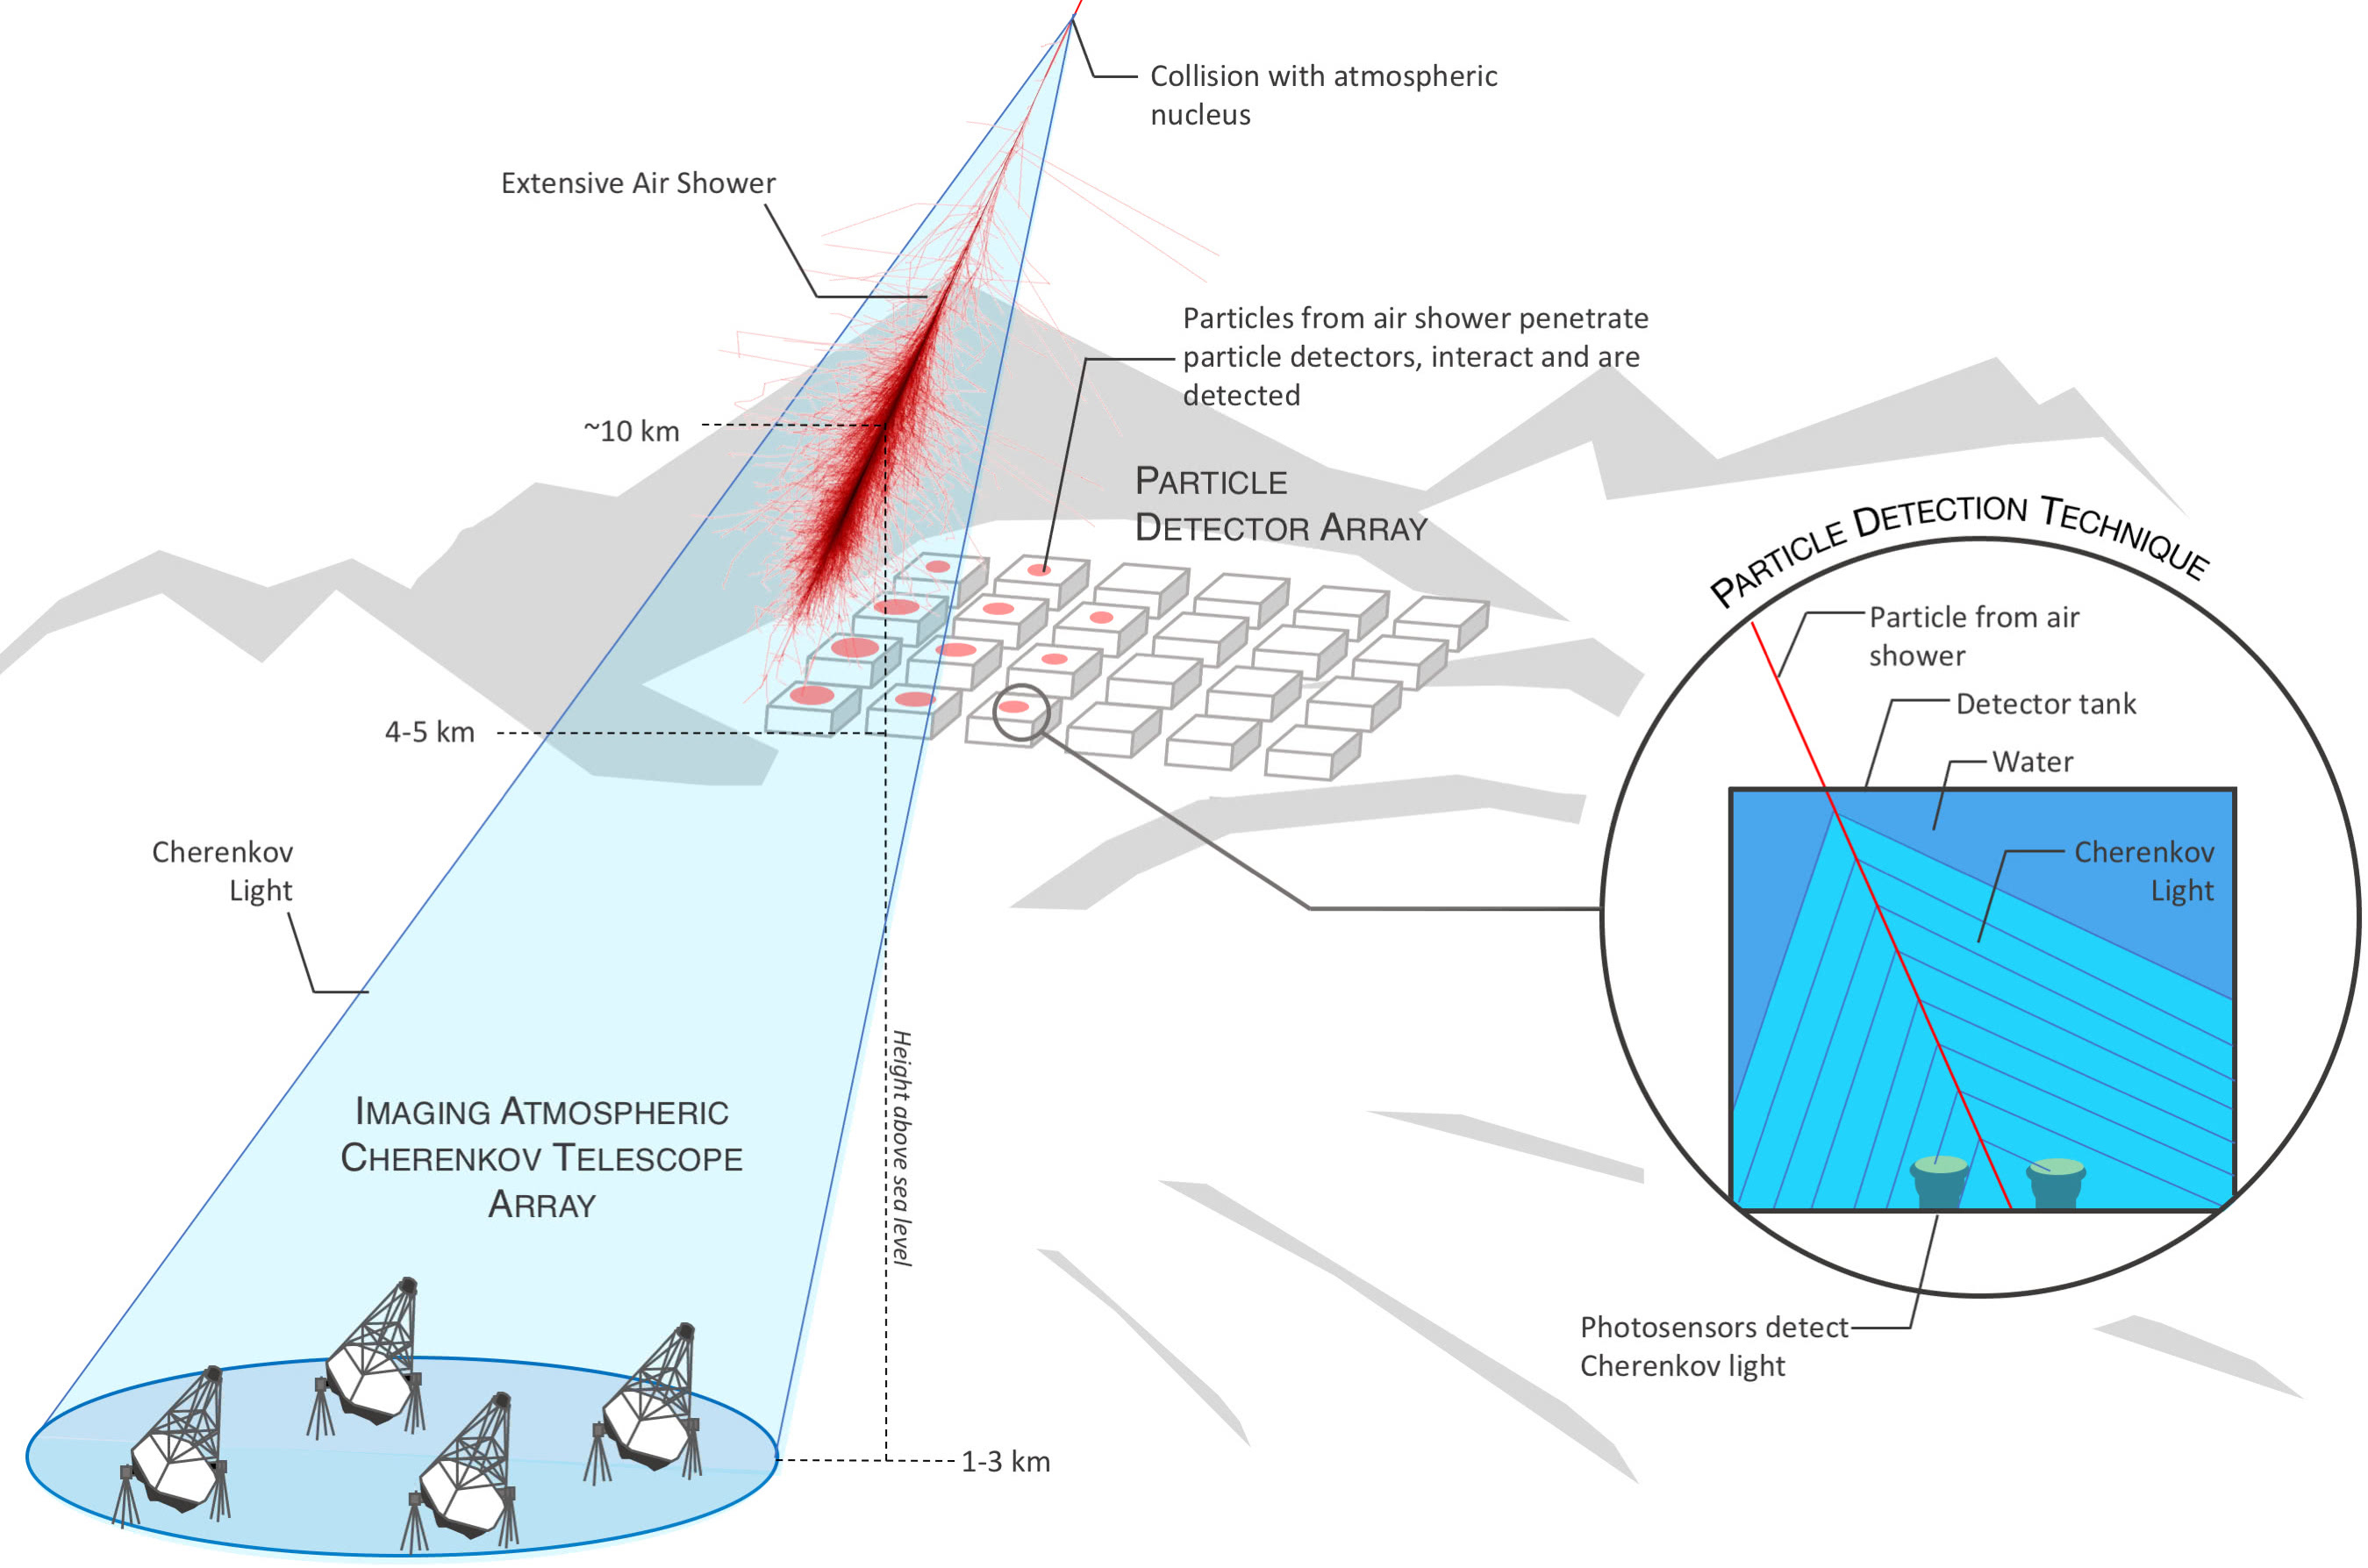
\includegraphics[width=\textwidth]{./images/detector_swgo.jpg}
        \caption{Direct particle detection at high altitudes with an extended air shower array and Imaging Air Cherenkov Telescopes at lower altitudes detecting the produced Cherenkov light in the atmosphere. \cite{SWGO19}}
        \label{fig:detect_swgo}
    \end{subfigure}
    \begin{subfigure}{0.7\textwidth}
        \vspace{0.5cm}
        \centering
        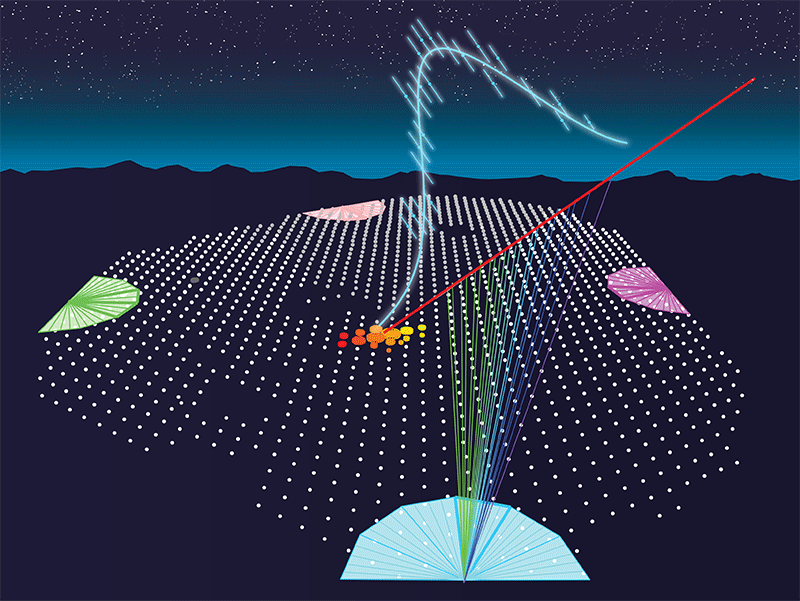
\includegraphics[width=\textwidth]{./images/detector_auger.png}
        \caption{Air shower measurement techniques of the Pierre-Auger Observatory using surface detectors and Fluorescence detectors. \cite{Gaisser16Auger}}
        \label{fig:detect_auger}
    \end{subfigure}
    \caption{Air shower measurement techniques using direct particle detection at high altitudes with an extended air shower array and the produced Cherenkov light in the atmosphere using Imaging Air Cherenkov Telescopes.}
    \label{fig:detect_air_shower}
\end{figure}

\subsection{Cosmic-Ray induced Air Shower Detectors}

Also at these moderate altitudes, it is possible to measure the fluorescence light produced mainly by the electromagnetic component of an air shower.
As these fluorescence detectors can cover a large effective area, rare events like the cosmic-rays at the GZK cut-off can be measured.
Currently, the most sensitive experiments for this type of detection are the Telescope Array \cite{TA12FD, TA13SD} in Utah observing the northern hemisphere and the Pierre Auger Observatory \cite{Auger15} in Argentina for the southern hemisphere both operating at around \SI{1400}{m} asl.
The Pierre Auger Observatory, shown in \figref{fig:detect_auger} consists of 24 fluorescence telescopes and 1500 Water Cherenkov Tanks on an area of \SI{300}{\square\kilo\meter} each containing \SI{12}{\cubic\meter} water and 3 PMTs.

Combining the fluorescence detection with an array of surface detectors sparsely placed on a large area to measure the particles reaching the ground has become a successful approach to measure the highest cosmic-rays.
In this hybrid method, the fluorescence detectors measure the longitudinal profile of the shower and thereby the energy of the shower.
The surface detectors measure the electromagnetic component only for vertical showers or just the muonic component for inclined showers being sensitive to the mass composition of the cosmic-ray.
While the surface detectors have a full duty cycle, the fluorescence detectors can only operate at clear nights, similar to the IACTS and EAS-Arrays and their duty cycles.
In combination with the lateral shower profile and its arrival times measured by the surface detectors, the main information of the primary particle, composition, energy and direction can be reconstructed.
Unfortunately, discrepancies in the number of muons between the measurement and the prediction of the simulation limit the use of Monte-Carlo based analysis and therefore the sensitivity on the mass composition.

Recent developments for the Pierre Auger Observatory \cite{Auger16Prime, Castellina19Prime} also include the usage of scintillator detectors at the surface, which are more sensitive to the electromagnetic component while being less sensitive to the nearly horizontal propagating muons of inclined showers.
Also part of this upgrade is placing radio antennas at each station to detect the radio signal thus measuring more components of the shower to better reconstruct the particle shower.

\subsection{Further Detectors measuring Atmospheric Muons}

A transit between a cosmic-ray induced muon detector and a neutrino detector is the NEjtrinnyj VOdnyj (Water) Detektor, NEVOD \cite{NEVOD15} located inside a building  at the MePhI in Moscow.
The detector, shown in \figref{fig:detect_nevod}, consists of a water-filled chamber with a size of $\SI{9}{m} \times \SI{9}{m} \times \SI{26}{m}$.
Inside this indoor pool, 25 Strings each containing three or four Quasi-Spherical-Modules which themselves consist of six PMTs looking in all three orthogonal directions, forward and backward and measure the light of the muons propagating through the chamber.
Due to the three-dimensional detector structure, the muons are not just registered, but also their energy loss behavior can be measured.
To increase the angular resolution for horizontal events, the DECOR enhancement was built consisting of streamer tube chambers at the sidewalls of the detector.
The high sensitivity on horizontal air showers and muon bundles makes this detector unique to analyze atmospheric muons and the Muon-Puzzle.
Next to the measurement of atmospheric air showers, NEVOD can detect neutrinos selecting upward-going events.
\begin{figure}
    \centering
    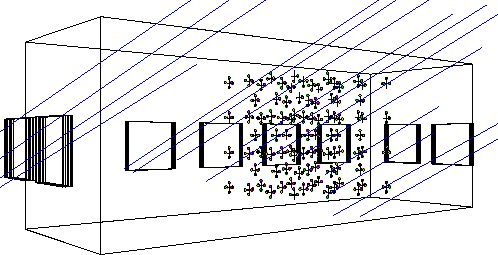
\includegraphics[width=\textwidth]{./images/detector_nevod.pdf}
    \caption{Sketch of the NEVOD-DECOR detector consisting Quasi-Spherical-Modules. \cite{NEVOD18}}
    \label{fig:detect_nevod}
\end{figure}

Another field of research detecting atmospheric muons with applications outside of the particle physics is the muon tomography.
Using the attenuation of the muon flux that varies between different materials, larger volumes of unknown material can be detected.
Application areas are the detection of varying magma chambers leading to a prediction of an eruption sequence of a volcano \cite{Tanaka09} or the detection of an unknown chamber in the Cheops pyramid \cite{Morishima17}.
Further applications are the measurement of large-angle Coulomb scattering to detect materials with high atomic numbers \cite{Borozdin03}.
Those detectors consist of several layers of plastic scintillators with the size of some \si{m^2} each passing the light to an SiPMs to track the number of muons and their direction.
An overview of the current muon imaging tools is reviewed in \cite{Bonechi19}.

So far, only experiments at the surface have been discussed measuring the muonic shower component as part of the signal or the main signal.
For most experiments located deep underground atmospheric muons are considered as background and not used to study cosmic ray physics, but to search for rare events like proton decays or Dark Matter interactions.
An exemplary detector for Dark Matter is the PICO detector \cite{Amole19PICO} in the Sudbury mine in Canada \SI{2}{km} below the surface, which equals \SI{6}{kmwe}.
Inside a pressure vessel with a diameter of \SI{60}{cm} and a height of \SI{167}{cm} superheated liquid C$_3$F$_8$ is used to measure small recoil energies (\SIrange{1}{100}{keV}) induced by elastic scattering of Weakly Interacting Massive Particles (WIMPs), a candidate for Dark Matter.
The main background limiting the sensitivity is not the atmospheric muons themselves, but the neutrons produced in interactions near the detector after propagating all the way down.
For these types of experiments, a precise description of the angular and energy distribution of the muon flux is crucial, especially the probability to reach those depths for inclined muons traveling even greater distances through the rock.
Therefore, the physical models need to be calculated and simulated with high precision, even for the edge cases of the stochastic propagation.
An exemplary detector for proton decay was the Fr\'{e}jus-Detector \cite{Frejus95nu} located \SI{4800}{mwe} under the Col du Fr\'{e}jus.
The calorimetric detector of the size () used iron to track particle interactions inside the detector.
Although a proton decay had not been measured, atmospheric muons had been used to create a depth curve and also the energy spectrum of atmospheric neutrinos had been unfolded.

%
%
% small seperation between the chapters
%
%

\section{Neutrino Detectors}

Besides the NEVOD Detector, most neutrino detectors are located deep underground to exclude the dominating background of atmospheric muons.
The low interaction rate of neutrinos is on the one side an advantage as it increases the observable horizon and let them propagate even through dense media like the core of the earth.
On the other side, this makes them challenging to detect and a large volume of detector material is required.
Due to the steep power-law dependence of the energy flux the energy range of the neutrinos scales with the size of the detection volume.
Four main types of neutrino telescopes have been established so far.

%  use the Cherenkov light emitted by charged secondary particles to measure neutrinos.
% Large volumes of media transparent to the blue Cherenkov light like Water, Ice or simply the air is used as a detection volume.
% Other methods like the radio or acoustic detection are in the development phase.

\subsection{Neutrino Telescope Types}

An exemplary detector in the neutrino energy range from MeV to \SI{10}{GeV} is the Super-Kamioka Neutrino Detection Experiment \cite{HyperKamiokande18} located in a former mine \SI{1}{km} deep underground in Japan.
It consists of a cylindrical tank with \SI{40}{m} in diameter and height filled with \SI{50}{kt} of purified water.
The Cherenkov light produced by particles interacting inside this tank is measured with \num{13000} PMTs positioned at the walls.
This peripheral detector type is used, since the absorption length of the Cherenkov radiation is larger than the detector size.
Similar structures for this energy range are SNO \cite{SNO20}, BOREXINO \cite{Borexino09} and JUNO \cite{JUNO19}, all located deep underground with several kt of liquid and transparent detector material, water or liquid scintillator and the PMTs at the walls.

To detect neutrinos with energies above \SI{10}{GeV} larger detector volumes with an effective radius of $\mathcal{O}(\SI{100}{m})$ are required.
These volumes can just be reached by using natural resources and placing the detectors inside the water, i.e. glacial ice, deep lakes or the sea.
Those distances exceed the absorption lengths of the Cherenkov light for water and a lattice structure of the detector is used.
Currently, the largest and most sensitive detector is the IceCube Neutrino Observatory at the South Pole with a detection volume of a cubic kilometer, which is further described in section \ref{sec:IceCube}.
Inside a detection volume of a cubic kilometer, the Cherenkov light produced by neutrinos or atmospheric muons is measured with around 5000 PMTs.
Therefore this type of telescope is labeled \textit{Cherenkov Neutrino Telescope}.
Further neutrino telescopes using the detection principle like IceCube are the ANTARES/Km3Net \cite{ANTARES11, KM3Net16} experiment in the Mediterranean sea, the Baikal/GVD in Lake Baikal \cite{Baikal97, GVD19} and the P-ONE experiment in the Cascadia Bassin in front of Vancouver \cite{PONE20}.
Compared to IceCube these telescopes are all upgrading to a volume of a cubic kilometer, are all located in the northern hemisphere and all use liquid water as detection volume.
Although the detection media is always water-based, the propagation of the Cherenkov light mainly described by the scattering and absorption differs significantly, as shown in \tabref{tab:len_abs_scat}.
While a strong absorption leads to the loss of photons and worse energy measurements, a strong scattering delays the photons and leads to a loss of directional information.
\begin{table}
    \caption{Characteristic lengths of absorption $\lambda_{\text{abs}}$ and scattering $\lambda_{\text{scat}}$ for selected locations with a Cherenkov-based neutrino detector. For detectors in liquid water, the range indicates the seasonal variation. The scattering lengths are corrected for the average Mie-Angle of the medium $\lambda_{\text{eff}}=\lambda_{\text{scat}}/(1-\langle\cos \theta\rangle)$. (TODO: cite private communication from Olga at Astropatricle School 2016 in Bad Honnef, find better source)}
    \label{tab:len_abs_scat}
    \begin{center}
    \begin{tabular}{l c c c}
        \toprule
        Location & Depth / km & $\lambda_a$ / m & $\lambda_{\text{eff}}$ / m \\
        \midrule
        Lake Baikal & $\sim 1$ & 22 & 150-400 \\
        Mediterranean Sea & $> 1.5$ & 40-70 & 200-400 \\
        South Pole & $1.5 - 2$ & 110 & 25 \\
        South Pole & $2 - 2.5$ & 220 & 47 \\
        \bottomrule
    \end{tabular}
    \end{center}
\end{table}

With this type of neutrino telescopes neutrinos with energies up to \SI{10}{PeV} can be measured.
Also with the planned IceCube-Gen2 detector increasing the size by a factor of ten \cite{IceCube20Gen2} the expected flux of the highest energetic neutrinos is too low to be detectable.
However, similar to the Pierre-Auger Observatory a maximum size of this type of detector is reached with Gen2.
To detect even higher energetic neutrinos and analyze the predicted cosmogenic neutrinos, detectors measuring the radio signal are under development.
Because of the long wavelength, these radio pulses can propagate several kilometers through the ice.
Therefore these detectors can be placed sparsely and cover a cubic kilometer with just a single station.
There are currently two attempts to build a Radio-Neutrino Detector; one as part of IeCube-Gen2 in the Antarctic Ice and another one on Greenland \cite{RNOG20}.

Another approach to measure neutrinos is looking for showers coming from Earth as just neutrinos can propagate through the Earth.
The ANITA experiment consists of radio antennas on a balloon.
During the flights around the Antarctic circle, it measures the radio signals coming from the Earth.
Pierre Auger is looking for showers going upward for extremely inclined showers.
If they measure not just the muon component but also the electromagnetic shower inside their surface detectors, the shower must have started deep inside the atmosphere, which only neutrinos can create.
HAWC looks at showers coming from neighboring mountains and MAGIC looks at the Atlantic if the view to the stars is not clear but the view to the sea.
Both again looking for a hadronic shower, only Tau Neutrinos can produce.
For all these experiments again atmospheric muons are the dominant background by orders of magnitudes.
Therefore an accurate description for all energies and energy losses is crucial to cover also the edge cases in the simulations.

\subsection{IceCube} \label{sec:IceCube}

The biggest neutrino telescope is the IceCube detector located at the geographic south pole, shown in \figref{fig:icecube_detector}.
On a hexagonal grid of a square kilometer, 78 Strings are drilled into the glacial ice with a string distance of \SI{125}{m}.
Each string contains 60 Digital Optical Modules (DOMs) equally placed between a depth of \SI{1500}{m} and \SI{2500}{m}.
Each DOM contains a Photomultiplier looking downward and measuring the emitted Cherenkov light of muons and neutrino interactions.
The surrounded detection volume contains a cubic kilometer of ice measuring neutrino energies between \SI{100}{GeV} and \SI{10}{PeV}.
For higher energies, the event rate is too small and for lower energies, the string spacing is too large.
\begin{figure}
    \centering
    \begin{subfigure}[t]{0.58\textwidth}
        \centering
        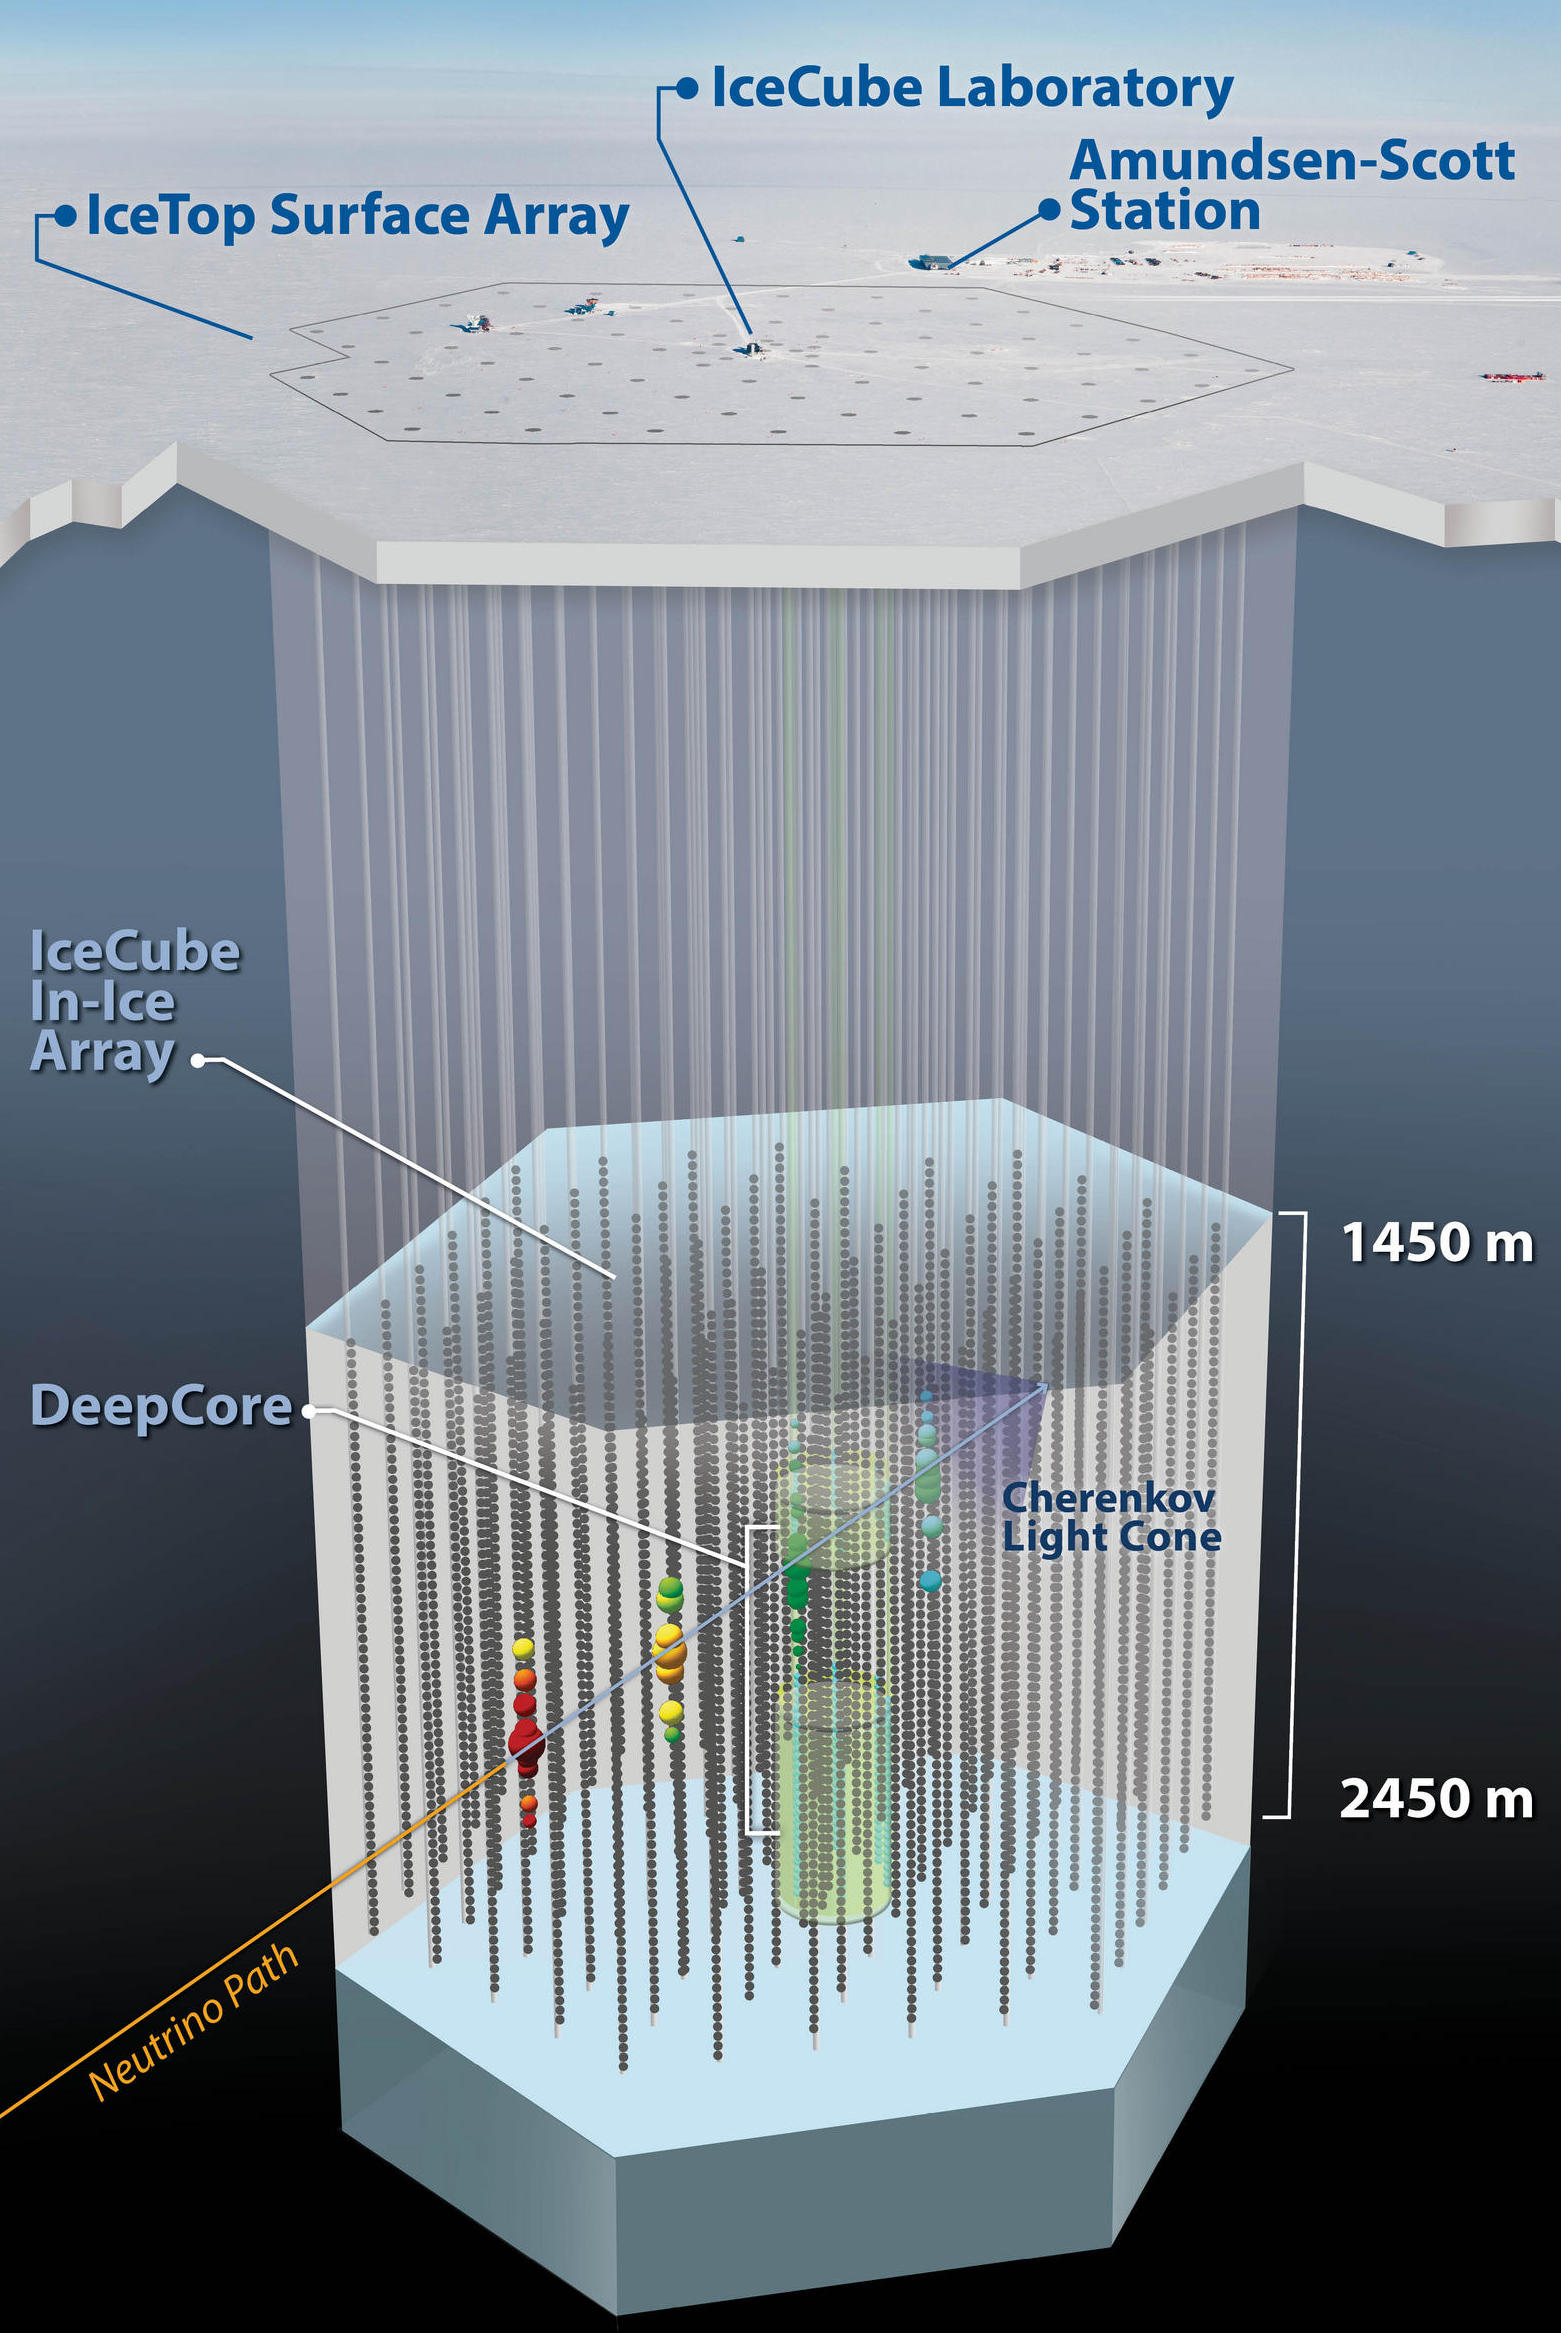
\includegraphics[width=\textwidth]{./images/icecube_detector.jpg}
        \caption{Sketch of the IceCube facilities at the South Pole and how an event view of a muon neutrino could look like. \cite{IceCubePics}}
        \label{fig:icecube_detector}
    \end{subfigure}
    \hfill
    \begin{subfigure}[t]{0.38\textwidth}
        \centering
        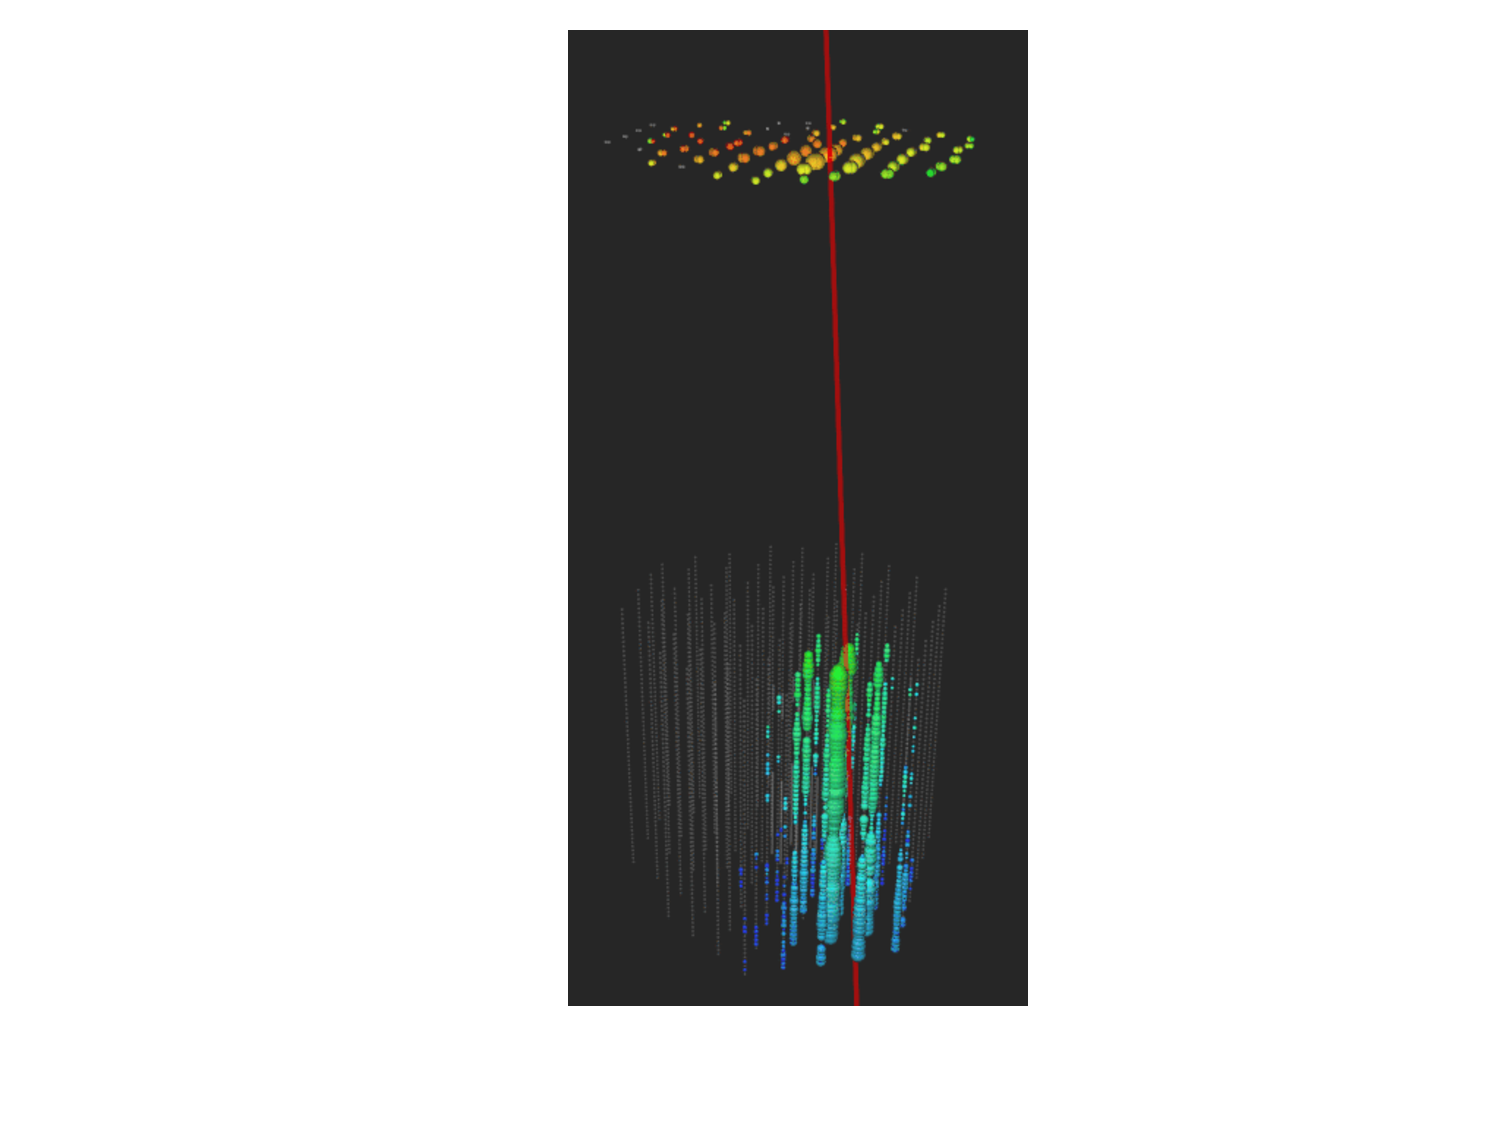
\includegraphics[width=\textwidth]{./images/icecube_event_300_pev_2010_07_02.pdf}
        \caption{Event view of a measured cosmic ray event in IceTop and IceCube on 02.07.2010 with a reconstructed primary particle energy of \SI{300}{PeV}. \cite{IceCubePics}}
        \label{fig:icecube_event_view}
    \end{subfigure}
    \caption{The IceCube Neutrino Observatory including the IceTop Array at the surface, the main in-ice detector and the DeepCore extension. For the event views, each colored circle indicates a DOM that measured light. The color ranges represents the time from red, early to blue, late. The size of the DOMs scales with the amount of detected light.}
    \label{fig:icecube}
\end{figure}

In the middle of IceCube 8 Strings, each with 60 DOMs of higher quantum efficiency are placed more densely together.
This extension called \enquote{DeepCore} decreases the lower threshold for neutrino energies to \SI{10}{GeV} and uses the rest of IceCube as a veto region.
Another extension is \enquote{IceTop} where a water Cherenkov tank is placed at the surface of each string.
This can either be used as an air shower detector at an altitude of \SI{3}{km} with the benefit of IceCube as a further muon detector to deeper analyze the atmospheric muons.
On the other side, it works as a veto for IceCube to distinguish down-going neutrinos from atmospheric muon events as the neutrinos should not be seen in IceTop.

There are currently plans for an extension of IceCube named IceCube-Gen2 \cite{IceCube20Gen2}.
The planned detector is shown in \figref{fig:detect_gen2}.
An extension called \enquote{IceCube-Upgrade} has already been funded to test new types of DOMs for Gen2.
Gen2 will enlarge the detected volume to \SI{8}{\cubic\kilo\meter} and will be placed around IceCube.
In contrast to IceCube, the Strings in Gen2 will be organized on a sunflower structure avoiding corridors where muons can sneak inside the inner volume and mimic a starting event.
Besides, a radio detector is planned, placing the antennas on a grid with an inner distance of a kilometer covering an area of \SI{100}{\cubic\kilo\meter} to analyze the cosmogenic neutrinos.
\begin{figure}
    \centering
    \includegraphics[width=\textwidth]{./images/gen2_detector.pdf}
    \caption{Schematic top view of the IceCube detector compared to the enhancements for Gen2. \cite{IceCube20Gen2}}
    \label{fig:detect_gen2}
\end{figure}

A distinct astrophysical neutrino source has also not been measured yet as well as a class of sources in a stacked search \cite{IceCube20PointSource, IceCube17BlazarStacking}.
However, a coincidence of a high energy neutrino event originating from the same direction as an AGN flaring at the same time in the gamma energy region is the first hint of a possible neutrino source \cite{IceCube18MMA, IceCube18TXS}.

\subsubsection{Event Signatures}

The measured event signatures are mainly divided into tracks and cascades.
A long track signature of an atmospheric muon bundle is shown in \figref{fig:icecube_event_view}.
Tracks are long, nearly straight lines along the muon path with the energy losses along the track producing the track signature.
Due to their long range, they can be further classified into starting, stopping, through-going and corner clippers.
Only neutrinos can produce starting events and stopping events can only be produced by a huge stochastic loss, which happens rarely or by low energetic muons.
Most-often, muons propagate through the detector producing a long path along their track.
There is however the special case of a corner clipper, that can mimic a cascade-like event at the edge of the detector.

A particle shower created by a single particle interaction (or multiple interactions inside a small range of less than \SI{10}{m}, which is pint-like for IceCube), produces a rather spherical spread of the produced Cherenkov light.
Although the particle cascade is boosted in the forward direction with just small transversal momentum and a Moli\`{e}re radius in the ice of \SI{10}{cm} \cite{PDG20}, the small scattering length creates a spherical propagation of the produced Cherenkov light.

NC-interactions of all neutrino flavors have just a visible hadronic shower, as the incoming and outgoing neutrino doesn't produce a signal, thus producing a single cascade.
Regarding CC interactions and starting with the electron neutrino, the additional electron loses most of its energy in less than \SI{10}{m} in the ice.
As this distance is point-like for IceCube, the resulting cascade also has a spherical structure.
Although there are differences in the shower developments of electromagnetic and hadronic cascades, especially through the later decays of neutral hadrons, it was not possible yet to distinguish between electromagnetic and hadronic cascades \cite{Steuer17ICRC}.

The greater mass of muons compared to electrons makes them lose their energy much slower and let them travel several kilometers through the ice.
From the hadronic cascade at the neutrino interaction vertex, a long track is going out.
Therefore muon neutrinos do not have to interact inside the detection volume and can also interact far before the detector with the muons traveling inside, increasing the effective detector volume.

Tau leptons have an even higher mass compared to the muons and have therefore a smaller energy loss resulting in a thin propagation track.
But the small lifetime of \SI{290}{fs} makes them decay directly or for higher energies let them just travel \SI{50}{m} per PeV.
The event signature depends on the decay channel; two-thirds are the hadronic decay channel and the last third is equally distributed between the muonic and the electronic channel.
Until energies of around \SI{10}{TeV} the second hadronic or em-cascade can not be distinguished from the first hadronic cascade at the neutrino vertex.
For higher energies first, a double pulse waveform at a single DOM can be registered and later these two cascades get separated more clearly and a double cascade or double bang signature is created.

The muonic tau decay also contributes to the amount of incoming muons starting before the detector.
For events starting inside the detector, the outgoing track is smaller compared to the hadronic cascade as the additional neutrinos from the tau decay take away some energy.
For higher energies, the thin tau track goes over to a brighter muon track.
But these differences in the track signature can just be separated statistically for many events and not on an event level due to the stochasticity of the propagation.
Due to the limited resolution, there has been just one promising tau neutrino event seen with IceCube after 10 years of measurement \cite{Meier19ICRC, IceCube20HeseTau}.

\subsubsection{Event selections}

The main interesting features to be reconstructed are the primary particle type, its energy and the direction.
To extract the primary particle type a classification of the different event signatures is required.
For these selections, multivariate methods are required since the atmospheric muon rate of \SI{1}{kHz}, is many orders above the atmospheric neutrino rate of \SI{1}{mHz} or the astrophysical neutrino rate of \SI{1}{\micro.Hz}.

A pure \textbf{cascade sample} contains mostly CC interacting electron neutrinos, fewer NC events and a few tau neutrinos.
Cascade searches \cite{IceCube20Cascades} uses the outer DOM layers as veto region against through-going muons, which have a detection rate that is multiple orders of magnitudes higher.
But even in DeepCore, muon tracks are contaminating the cascaded selections when traveling in the middle between the strings due to the lattice structure.
Also, the stochasticity of the propagation processes, allowing muons to travel without visible losses and then deposit all of their energy in a catastrophic loss inside the detector limits the selection efficiency.
As these processes are rare, an accurate description of the muon physics even at the tails or edges of the total and differential cross section is needed.
These selection methods are not just valid for cascades, but all kind of starting events.

The tracks are further separated between up-going and down-going tracks.
Down-going events are most-often atmospheric muons reaching the detector as bundles with a lateral distance of some meter between them.
Those events are seen as one thick, bright track due to the limited resolution preventing a separation of the single muons from a bundle.
Therefore those muon bundles are in principle of limited usefulness since the number of muons and their energy is not reconstructible.
An approach to analyzing atmospheric muon bundles is the search for a \textbf{leading muon} containing most of the bundle energy \cite{Fuchs16PhD}.
A bundle of many low energetic muons creates a bright track with a continuous energy loss.
Leading or single muons have higher stochasticity, e.g. with a huge bremsstrahlung loss resulting in a thinner track with brighter cascades along it.
As these muons are produced in one of the first interactions of the air shower they can provide further insights into the particle processes in the atmosphere.

Another approach to use atmospheric muons is using \textbf{stopping muons} \cite{Hoinka17Master}.
They are most-often single muons and have energies of just several \SI{100}{GeV} when entering the detector.
At these energies, they are in the regime of the minimal Ionization and can be used to calibrate the detector and measure systematic parameters.
For stopping muons, also the range they have traveled through the ice is known which is an approximation of their energy at the surface.
Therefore they can also be used to study cosmic ray and air shower physics, but in comparison to the leading muons for higher energies, stopping muons provide insights at lower energies.

\textbf{Up-going muon tracks} can only be neutrino-induced muons as muons cannot propagate large distances through the earth.
Unfortunately, a simple extraction of these muons with a zenith cut is not satisfying as the resulting sample is still dominated by mis-reconstructed muons.
Although the directional resolution is high for tracks, sometimes it can exceed \SI{5}{\degree} and contaminate the sample.
Therefore advanced machine learning algorithms are used to extract a purified sample \cite{Stettner19ICRC}.
The filtered track events are an ideal single muons sample at all energies; good to analyze the muon physics, e.g. the energy loss profile.
Just for the starting events, the hadronic cascade of the neutrino interaction contaminates a little bit.

\subsubsection{Event Reconstruction}

After the selection, the energy and directional reconstruction is the remaining step before analyzing the desired event sample.
An overview of the standard reconstruction methods is given in \cite{AMANDA2004Reco, IceCube2014Ereco}.
In recent years also modern, machine-learning-based methods using e.g. Deep Neural Networks have been developed increasing the accuracy of the reconstruction \cite{Huennefeld17ICRC, Huennefeld17Master, IceCube20DNN}.
A comparison of the standard and neural network approaches for the reconstructions is shown in \figref{fig:icecube_reco} as well as their energy dependence.
\begin{figure}
    \centering
    \begin{subfigure}{0.55\textwidth}
        \centering
        \includegraphics[width=\textwidth]{./images/icecube_cascade_angular_resolution.pdf}
        \caption{Resolution of the angular reconstruction for cascades comparing the standard likelihood approach with a Neural Network (CNN). \cite{IceCube20DNN}}
        \label{fig:icecube_angular_resolution}
    \end{subfigure}
    \hfill
    \begin{subfigure}{0.43\textwidth}
        \centering
        \includegraphics[width=\textwidth]{./images/icecube_muon_energy_resolution.pdf}
        \caption{Resolution of the energy reconstruction for tracks comparing the standard $\mathrm{d}E/\mathrm{d}X$ and track length approach with a Deep Neural Network. \cite{Huennefeld17Master}}
        \label{fig:icecube_energy_resolution}
    \end{subfigure}
    \caption{Energy dependence of the resolution of the challenging reconstruction parameters in IceCube. On the left the angular reconstruction for cascades and on the right the energy reconstruction for tracks is compared between modern neural network approaches and the default likelihood approaches.}
    \label{fig:icecube_reco}
\end{figure}

The directional resolution for tracks is comparably high (\SI{0.5}{\degree}) while being low for cascade events (\SI{15}{\degree}).
Regarding the energy reconstruction, it's the other way round.
When a cascade is contained inside the detector the energy resolution is high due to the calorimetric measurement resulting in an uncertainty of \SI{10}{\%}.
For through-going tracks, just a portion of the muon energy loss is deposited inside the detector
For muons above a TeV the energy is reconstructed using the average energy loss per distance $\mathrm{d}E/\mathrm{d}X$, which increases nearly linear with the muon energy (c.f. section \ref{sec:dedx}).
Therefore, the track inside the detector is split into multiple segments and the high energetic, stochastic losses are cut away to extract the continuous energy loss.
The energy resolution 
For starting tracks, the energy resolution of the muons and neutrinos improves, due to the additional information of the hadronic cascade at the vertex.
For low energy muons, the average energy loss is not proportional to the muon energy.
As these muons are most-often stopping inside the detector, the track length can be used to reconstruct the energy.

Next to the energy and direction, also the energy losses along a muon track can be reconstructed, which is important for analyses depending on the stochasticity, e.g. when creating a leading muon sample.
Since IceCube cannot distinguish between single energy losses, the track inside the detector is split into multiple segments as for the $\mathrm{d}E/\mathrm{d}X$ energy reconstruction and the energy loss in each segment unfolded.
This is just sensitive to high stochastic energy losses and can be used to study the energy loss profile of the muons.

The last important topic regarding event reconstructions is the systematic uncertainty.
In every experiment, some remaining parameters are challenging to calibrate or measure and have uncertainties that are non-negligible for analyses.
For the IceCube detector, one main systematic parameter is the quantum efficiency of the DOMs, short DOM efficiency.
This varies the amount of detected light and has an uncertainty of $\pm\SI{5}{\percent}$.
The other main uncertainties are the ice properties, mainly the absorption and scattering lengths, which are depth-dependent.
The depth dependence does not originate due to the different levels of pressure and thus temperature, but due to several layers of dust \cite{Icecube06ice, Icecube13ice}.
Especially in the middle of the detector at a depth around \SI{2}{km} the absorption length is significantly decreased and nearly all photons get absorbed before reaching a DOM.
This blind layer is slightly indicated in \figref{fig:icecube_event_view}.
Further systematics of the glacial ice like the anisotropy are discussed in detail in \cite{Rongen19PhD}.

Next to these detector and ice properties, further sub-dominant systematics arise due to the theoretical uncertainties of the physical processes.
Regarding the muon physics, the uncertainties of the cross sections needs to be differentiated between the processes dominant for the low energy losses and processes dominating the high, stochastic energy losses.
While an increase of the low energy losses can already be compensated by an increase in the DOM efficiency, the uncertainties of the stochastic energy losses have not been considered, yet.
Since the stochasticity of the muon affects the performances of separating leading muon, cascade or tau samples, an approach to include them is analyzed in this work.

To take into account all of these systematics, simulation sets each varying one or two systematic parameters on a grid and interpolations between these grid points were used in analyses.
However, this grid approach increases the number of required simulation sets for every further systematic parameter resulting in the curse of dimensionality.
There is now a new approach \cite{IceCube2019SnowStorm} where for each simulation run a new set of all systematic parameters is sampled from their uncertainty distribution, including correlation.
With this Monte-Carlo approach, the phase space can be filled also when including further systematics.
